\documentclass{ximera}

\title{Change of Variables in Multiple Integrals}
\author{Zack Reed}

\begin{document}
\begin{abstract}
In this activity we explore how to change coordinate systems in multiple integrals, extending u-substitution from single-variable calculus to transformations in higher dimensions.
\end{abstract}
\maketitle

\section*{Introduction: Why Change Variables?}

In single-variable calculus, u-substitution transformed difficult integrals into easier ones. For multiple integrals, changing coordinate systems serves the same purpose!

\begin{problem}
Recall u-substitution from Calculus I:
$$\int f(g(x)) g'(x)\,dx = \int f(u)\,du \text{ where } u = g(x)$$

The key insight: \wordChoice{\choice{We make the integral harder}\choice[correct]{We transform to simpler coordinates}\choice{We change the function}}

What's the role of $g'(x)$?
\begin{multipleChoice}
    \choice{It makes the problem harder}
    \choice[correct]{It accounts for how $dx$ transforms to $du$}
    \choice{It's optional}
    \choice{It cancels out}
\end{multipleChoice}

\begin{feedback}
The derivative $g'(x)$ accounts for the ``stretching'' or ``compression'' when we change variables! In multiple dimensions, we'll need something similar.
\end{feedback}
\end{problem}

\section*{Revisiting a Problem: From Cartesian to Cylindrical}

\begin{problem}
\textbf{Example: Mass Under a Paraboloid (Revisited)}

In the last module, we encountered this problem: Find the mass of a solid bounded below by the $xy$-plane and above by the paraboloid $z = 4 - x^2 - y^2$, with a circular base of radius 1, if the density is $\rho(x,y,z) = z$ (denser at higher altitudes).

\begin{center}
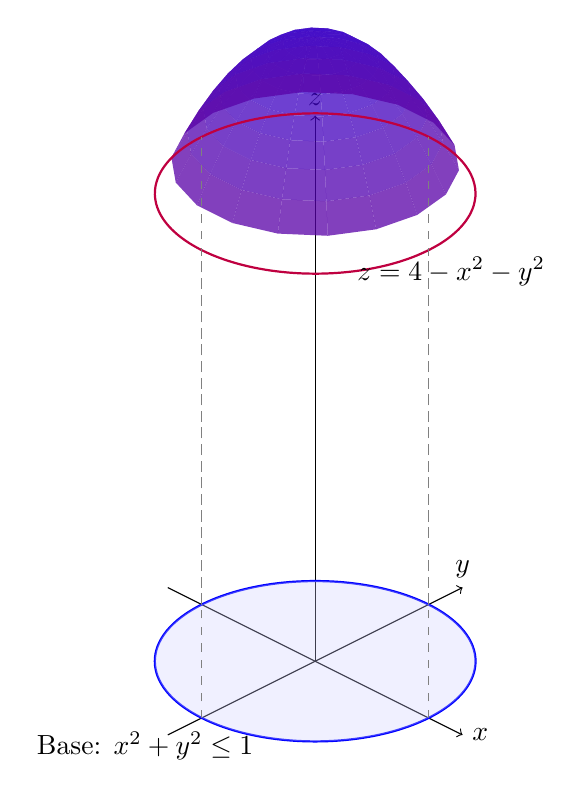
\begin{tikzpicture}[x={(0.8cm,-0.4cm)}, y={(0.8cm,0.4cm)}, z={(0cm,1.1cm)}, scale=1.8]
    % Draw axes
    \draw[->] (-1.3,0,0) -- (1.3,0,0) node[right] {$x$};
    \draw[->] (0,-1.3,0) -- (0,1.3,0) node[above] {$y$};
    \draw[->] (0,0,0) -- (0,0,3.5) node[above] {$z$};
    
    % Draw the circular base
    \draw[thick, blue] (0,0,0) circle (1);
    \fill[blue!20, opacity=0.3] (0,0,0) circle (1);
    
    % Draw the paraboloid surface as a smooth cap
    \foreach \r in {0,0.1,...,0.9} {
        \pgfmathsetmacro{\rnext}{\r+0.1}
        \pgfmathsetmacro{\zr}{4-\r*\r}
        \pgfmathsetmacro{\zrnext}{4-\rnext*\rnext}
        \foreach \theta in {0,20,...,340} {
            \pgfmathsetmacro{\thetanext}{\theta+20}
            \pgfmathsetmacro{\xa}{\r*cos(\theta)}
            \pgfmathsetmacro{\ya}{\r*sin(\theta)}
            \pgfmathsetmacro{\xb}{\rnext*cos(\theta)}
            \pgfmathsetmacro{\yb}{\rnext*sin(\theta)}
            \pgfmathsetmacro{\xc}{\rnext*cos(\thetanext)}
            \pgfmathsetmacro{\yc}{\rnext*sin(\thetanext)}
            \pgfmathsetmacro{\xd}{\r*cos(\thetanext)}
            \pgfmathsetmacro{\yd}{\r*sin(\thetanext)}
            \pgfmathsetmacro{\cavg}{(\zr+\zrnext)/2*20}
            \fill[blue!\cavg!red, opacity=0.75] 
                (\xa,\ya,\zr) -- (\xb,\yb,\zrnext) -- (\xc,\yc,\zrnext) -- (\xd,\yd,\zr) -- cycle;
        }
    }
    
    % Draw boundary circle on top at r=1
    \draw[thick, purple, domain=0:360, samples=60, smooth, variable=\t] 
        plot ({cos(\t)}, {sin(\t)}, {3});
    
    % Draw some vertical edges for reference
    \draw[gray, dashed, thin] (1,0,0) -- (1,0,3);
    \draw[gray, dashed, thin] (-1,0,0) -- (-1,0,3);
    \draw[gray, dashed, thin] (0,1,0) -- (0,1,3);
    \draw[gray, dashed, thin] (0,-1,0) -- (0,-1,3);
    
    % Label
    \node at (0.6, 0.6, 2.5) {$z=4-x^2-y^2$};
    \node at (0, -1.5, 0) {Base: $x^2+y^2 \leq 1$};
\end{tikzpicture}
\end{center}

\textbf{Review: The Cartesian Approach}

Last module, we set this up in rectangular coordinates with order $dz\,dy\,dx$:

The region: $x^2 + y^2 \leq 1$ and $0 \leq z \leq 4-x^2-y^2$

\textbf{Bounds:}
\begin{itemize}
    \item $z$ bounds: $0 \leq z \leq 4-x^2-y^2$ (curved paraboloid!)
    \item $y$ bounds: $-\sqrt{1-x^2} \leq y \leq \sqrt{1-x^2}$ (messy square roots!)
    \item $x$ bounds: $-1 \leq x \leq 1$
\end{itemize}

\textbf{The mass integral:}
$$M = \int_{-1}^{1} \int_{-\sqrt{1-x^2}}^{\sqrt{1-x^2}} \int_0^{4-x^2-y^2} z\,dz\,dy\,dx$$

After the $z$ integration: 
$$M = \int_{-1}^{1} \int_{-\sqrt{1-x^2}}^{\sqrt{1-x^2}} \frac{(4-x^2-y^2)^2}{2}\,dy\,dx$$

This becomes quite complex! Those square root bounds and the $(4-x^2-y^2)^2$ term make this tedious.

\textbf{Recognizing the Pattern:}

Notice the key features:
\begin{selectAll}
    \choice[correct]{The base is circular: $x^2 + y^2 \leq 1$}
    \choice[correct]{The function involves $x^2 + y^2$}
    \choice[correct]{There's radial symmetry}
    \choice{The region is a rectangular box}
\end{selectAll}

When you see $x^2 + y^2$ and circular regions, think: \wordChoice{\choice{Rectangular}\choice[correct]{Cylindrical}\choice{Spherical}} coordinates!

\textbf{Step 1: The Cylindrical Transformation}

Cylindrical coordinates relate to Cartesian via:
\begin{align*}
x &= r\cos\theta\\
y &= r\sin\theta\\
z &= z
\end{align*}

The key observation: $x^2 + y^2 = \answer{r^2}$

And the volume element transforms: $dV = dx\,dy\,dz = \answer{r}\,dr\,d\theta\,dz$

\textbf{Step 2: Transform the Region}

The base $x^2 + y^2 \leq 1$ becomes: $r^2 \leq 1$, so $0 \leq r \leq \answer{1}$

The angle goes full circle: $0 \leq \theta \leq \answer{2\pi}$

The paraboloid $z = 4 - x^2 - y^2$ becomes: $z = 4 - r^2$

So: $0 \leq z \leq \answer{4-r^2}$

\textbf{Step 3: Transform the Density}

The density was $\rho(x,y,z) = z$

In cylindrical coordinates, this is still just: $\rho(r,\theta,z) = \answer{z}$

\textbf{Step 4: Set Up the Integral in Cylindrical Coordinates}

$$M = \int_{\answer{0}}^{\answer{2\pi}} \int_{\answer{0}}^{\answer{1}} \int_{\answer{0}}^{\answer{4-r^2}} z \cdot \answer{r}\,dz\,dr\,d\theta$$

Notice:
\begin{itemize}
    \item No more square roots!
    \item Simple constant bounds for $r$ and $\theta$
    \item The factor of $r$ accounts for the geometry
\end{itemize}

\textbf{Step 5: Evaluate the Integral}

\textbf{Inner integral ($z$):}
$$\int_0^{4-r^2} z\,dz = \left[\frac{z^2}{2}\right]_0^{4-r^2} = \frac{(4-r^2)^2}{2} = \answer{\frac{(4-r^2)^2}{2}}$$

Now we have:
$$M = \int_0^{2\pi} \int_0^1 \frac{(4-r^2)^2}{2} \cdot r\,dr\,d\theta$$

\textbf{Middle integral ($r$):}
$$\int_0^1 \frac{r(4-r^2)^2}{2}\,dr$$

Let $u = 4-r^2$, so $du = -2r\,dr$, or $r\,dr = -\frac{1}{2}du$

When $r=0$: $u = 4$; when $r=1$: $u = 3$

$$= \int_4^3 \frac{u^2}{2} \cdot \left(-\frac{1}{2}\right)\,du = \frac{1}{4}\int_3^4 u^2\,du = \frac{1}{4}\left[\frac{u^3}{3}\right]_3^4$$
$$= \frac{1}{12}(64-27) = \frac{37}{12}$$

\textbf{Outer integral ($\theta$):}
$$M = \int_0^{2\pi} \frac{37}{12}\,d\theta = \frac{37}{12} \cdot 2\pi = \answer{\frac{37\pi}{6}}$$

\begin{feedback}
By switching to cylindrical coordinates, we transformed a difficult integral with square root bounds into one with constant bounds! The circular symmetry of the problem made cylindrical coordinates the natural choice. This is the power of choosing the right coordinate system!
\end{feedback}
\end{problem}



\section*{Polar Coordinates}

For circular or radial regions, polar coordinates often simplify the integral dramatically.

\begin{problem}
Why use polar coordinates for integration?
\begin{selectAll}
    \choice[correct]{Circular regions have simpler bounds: $0 \leq r \leq R$, $0 \leq \theta \leq 2\pi$}
    \choice{Polar coordinates always make integrals easier}
    \choice[correct]{Functions with $x^2 + y^2$ simplify to $r^2$}
    \choice[correct]{Radial symmetry becomes apparent}
\end{selectAll}

\begin{feedback}
Polar coordinates are ideal when the region or function has circular/radial symmetry!
\end{feedback}
\end{problem}

\subsection*{The Polar Area Element}

\begin{problem}
The key question: What is $dA$ in polar coordinates?

\begin{expandable}{stuff}{GeoGebra Instructions}
    Use the ``Shift Radius'' and ``Shift $\theta$'' sliders to move the area element $dA$ around. Check ``Show Volume'' to see the approximating cylinder. Use ``Zoom to Unit Circle'' and drag to view from above.
\end{expandable}

\begin{center}
\geogebra{uucwvg4g}{740}{481}
\end{center}

The area element $dA$ is bounded between:
\begin{itemize}
    \item Circles of radius $r - \frac{dr}{2}$ and $r + \frac{dr}{2}$
    \item Angles $\theta - \frac{d\theta}{2}$ and $\theta + \frac{d\theta}{2}$
\end{itemize}

The area of this annular sector is approximately:
$$dA = \frac{d\theta}{2}(r+\frac{dr}{2})^2 - \frac{d\theta}{2}(r-\frac{dr}{2})^2$$

After algebra, this simplifies to: $dA = \answer{r} \cdot dr \cdot d\theta$

The extra factor $r$ is crucial! Without it:
\begin{multipleChoice}
    \choice{The integral would be easier}
    \choice[correct]{We'd get the wrong answer}
    \choice{Nothing would change}
\end{multipleChoice}

\begin{feedback}
The polar area element is $dA = r\,dr\,d\theta$. That extra $r$ accounts for the curved geometry!
\end{feedback}
\end{problem}

\begin{problem}
\textbf{Heat Distribution in a Circular Plate}

A circular metal plate of radius 3 meters has temperature $T(r,\theta) = 50 + 20\cos(2\theta)$ degrees Celsius, where $(r,\theta)$ are polar coordinates.

The heat energy density (energy per unit area) is $E(r,\theta) = cT(r,\theta)$ where $c$ is a constant.

\textbf{Construct the differential element carefully:}

In polar coordinates, the area element is: $dA = \answer{r}\,dr\,d\theta$

Why not just $dr\,d\theta$?
\begin{multipleChoice}
    \choice{It's a convention}
    \choice{To make the integral harder}
    \choice[correct]{The ``width'' of an angular slice is $r\,d\theta$, not $d\theta$}
    \choice{It's only true for circles}
\end{multipleChoice}

The small heat energy is: $dE = E(r,\theta) \cdot dA = c(50 + 20\cos(2\theta)) \cdot \answer{r}\,dr\,d\theta$

Total heat energy in the plate:
$$E_{\text{total}} = \int_{\answer{0}}^{\answer{2\pi}} \int_{\answer{0}}^{\answer{3}} c(50 + 20\cos(2\theta)) \cdot r\,dr\,d\theta$$

The temperature varies with $\theta$ but not $r$, meaning:
\begin{multipleChoice}
    \choice{The plate is hotter at the edge}
    \choice[correct]{Temperature varies around the circle but is constant along any ray from the center}
    \choice{The plate is uniformly heated}
    \choice{There's an error in the problem}
\end{multipleChoice}

\begin{feedback}
Great work! You recognized that in polar coordinates, the area element $dA = r\,dr\,d\theta$ accounts for the geometry. The factor of $r$ appears because angular slices get wider as you move away from the origin!
\end{feedback}
\end{problem}

\subsection*{Polar Integral Example}

\begin{problem}
Let's integrate $f(x,y) = xy$ over the unit disk $x^2 + y^2 \leq 1$.

\textbf{In rectangular coordinates (yuck!):}
$$\int_{-1}^1\int_{-\sqrt{1-x^2}}^{\sqrt{1-x^2}} xy\,dy\,dx$$

Those square root bounds are messy!

\textbf{In polar coordinates:}
\begin{itemize}
    \item Region: $0 \leq r \leq \answer{1}$, $0 \leq \theta \leq \answer{2\pi}$
    \item Function: $f(x,y) = xy = (r\cos\theta)(r\sin\theta) = \answer{r^2 \sin\theta \cos\theta}$
    \item Area element: $dA = \answer{r}\,dr\,d\theta$
\end{itemize}

The integral becomes:
$$V = \int_0^{2\pi}\int_0^1 r^2\sin\theta\cos\theta \cdot r\,dr\,d\theta = \int_0^{2\pi}\int_0^1 r^3\sin\theta\cos\theta\,dr\,d\theta$$

\textbf{Inner integral (with respect to $r$):}
$$\int_0^1 r^3\,dr = \left[\frac{r^4}{4}\right]_0^1 = \answer{1/4}$$

\textbf{Outer integral (with respect to $\theta$):}
$$\int_0^{2\pi} \frac{1}{4}\sin\theta\cos\theta\,d\theta = \frac{1}{4}\int_0^{2\pi} \frac{1}{2}\sin(2\theta)\,d\theta$$
$$= \frac{1}{8}\left[-\frac{1}{2}\cos(2\theta)\right]_0^{2\pi} = \frac{1}{8} \cdot 0 = \answer{0}$$

Why is the volume zero?
\begin{multipleChoice}
    \choice{We made a calculation error}
    \choice[correct]{The function $xy$ is negative in two quadrants and positive in two quadrants, so they cancel}
    \choice{The unit disk has zero area}
\end{multipleChoice}

\begin{feedback}
The symmetry of $xy$ means equal positive and negative volumes that cancel! Polar coordinates made this much cleaner to compute.
\end{feedback}
\end{problem}


\section*{Review: Polar Coordinates Revisited}

Let's examine what happens when we transform from rectangular to polar coordinates.

\begin{problem}
The transformation from polar to rectangular coordinates is:
\begin{align*}
x &= r\cos\theta\\
y &= r\sin\theta
\end{align*}

This transformation maps:
\begin{itemize}
    \item The $r\theta$-plane (polar) $\to$ The $xy$-plane (rectangular)
\end{itemize}

What happens to a small rectangle in the $r\theta$-plane?
\begin{multipleChoice}
    \choice{It stays a rectangle}
    \choice[correct]{It becomes a curved shape}
    \choice{It disappears}
    \choice{It becomes a circle}
\end{multipleChoice}

The area element transforms as:
$$dA = dx\,dy = \answer{r}\,dr\,d\theta$$

Why the factor of $r$?
\begin{selectAll}
    \choice[correct]{It accounts for the curved geometry}
    \choice[correct]{It measures how areas change under the transformation}
    \choice{It's arbitrary}
    \choice[correct]{It's the Jacobian determinant for this transformation}
\end{selectAll}

\begin{feedback}
The factor $r$ tells us how much a small area in the $r\theta$-plane expands or contracts when mapped to the $xy$-plane!
\end{feedback}
\end{problem}


\section*{Practice Problems}

\begin{problem}
Compute $\displaystyle\int_0^{\pi/2}\int_0^{\cos\theta} r^2\,dr\,d\theta$ in polar coordinates.

\textbf{Inner integral:}
$$\int_0^{\cos\theta} r^2\,dr = \left[\frac{r^3}{3}\right]_0^{\cos\theta} = \answer{\cos^3\theta / 3}$$

\textbf{Outer integral:}
$$\int_0^{\pi/2} \frac{\cos^3\theta}{3}\,d\theta = \frac{1}{3}\int_0^{\pi/2} \cos^3\theta\,d\theta$$

Using $\cos^3\theta = \cos\theta(1-\sin^2\theta)$ and substitution $u = \sin\theta$:
$$= \frac{1}{3}\left[\sin\theta - \frac{\sin^3\theta}{3}\right]_0^{\pi/2} = \frac{1}{3}\left(1 - \frac{1}{3}\right) = \answer{2/9}$$

\begin{feedback}
Great work! This integral computed the volume of a region bounded by a cosine curve in polar coordinates.
\end{feedback}
\end{problem}

\begin{problem}
Set up (but don't evaluate) the integral for the area of a circle of radius $R$ using polar coordinates.

Area formula: $A = \iint_R dA$

In polar: $A = \int_{\answer{0}}^{\answer{2\pi}}\int_{\answer{0}}^{\answer{R}} \answer{r}\,dr\,d\theta$

Evaluating quickly:
$$A = \int_0^{2\pi} \left[\frac{r^2}{2}\right]_0^R d\theta = \int_0^{2\pi} \frac{R^2}{2}\,d\theta = \frac{R^2}{2} \cdot 2\pi = \answer{\pi R^2}$$

Does this match the familiar formula? \wordChoice{\choice[correct]{Yes!}\choice{No}}

\begin{feedback}
Perfect! Double integrals can compute areas (by integrating $f=1$), volumes (by integrating $f(x,y)$), and many other quantities!
\end{feedback}
\end{problem}


\textbf{Mass of Fluid in a Rotating Container}

A cylindrical container (radius 2 m, height 5 m) rotates, causing the fluid density to vary:
$$\delta(r,z) = 1000 + 50r^2 - 20z \text{ kg/m}^3$$

where $(r, \theta, z)$ are cylindrical coordinates.

In cylindrical coordinates, the volume element is:
$$dV = \answer{r}\,dr\,d\theta\,dz$$

\begin{problem}

Why does $r$ appear here?
\begin{multipleChoice}
    \choice{It's always there in 3D}
    \choice[correct]{The cylindrical shell at radius $r$ has circumference $2\pi r$, making volume proportional to $r$}
    \choice{To account for rotation}
    \choice{It's a mistake}
\end{multipleChoice}

The small mass element: $dM = \delta(r,z) \cdot dV = (1000 + 50r^2 - 20z) \cdot \answer{r}\,dr\,d\theta\,dz$

The integral setup for total mass:
$$M = \int_{\answer{0}}^{\answer{2\pi}} \int_{\answer{0}}^{\answer{5}} \int_{\answer{0}}^{\answer{2}} (1000 + 50r^2 - 20z) \cdot r\,dr\,dz\,d\theta$$

Notice the density:
\begin{selectAll}
    \choice[correct]{Increases with distance from the axis (centrifugal effect)}
    \choice[correct]{Decreases with height (pressure effect)}
    \choice{Depends on angle $\theta$}
    \choice[correct]{Is independent of angle (axial symmetry)}
\end{selectAll}

\begin{feedback}
Perfect! You've unpacked $dM = \delta \cdot dV$ in cylindrical coordinates, recognizing that $dV = r\,dr\,d\theta\,dz$ reflects the geometry of cylindrical shells. The density function models realistic physical effects in a rotating container!
\end{feedback}
\end{problem}


\section*{Application: Mass of 3D Objects}

\begin{problem}
We'll work with two shapes with variable density:

\textbf{Shape 1 (Cone):} 
\begin{itemize}
    \item Height: 5 meters
    \item Base radius: 4 meters
    \item Density: $\delta = 3 + 2h$ kg/m$^3$, where $h$ is height from tip
\end{itemize}

\textbf{Shape 2 (Sphere):}
\begin{itemize}
    \item Radius: 5 meters
    \item Density: $\delta = 3 + 2\rho$ kg/m$^3$, where $\rho$ is distance from center
\end{itemize}

For the cone, which coordinate system is most natural?
\begin{multipleChoice}
    \choice{Rectangular $(x,y,z)$}
    \choice[correct]{Cylindrical $(r,\theta,z)$}
    \choice{Spherical $(\rho,\phi,\theta)$}
\end{multipleChoice}

For the sphere, which coordinate system is most natural?
\begin{multipleChoice}
    \choice{Rectangular $(x,y,z)$}
    \choice{Cylindrical $(r,\theta,z)$}
    \choice[correct]{Spherical $(\rho,\phi,\theta)$}
\end{multipleChoice}

\begin{feedback}
Choose coordinates that match the geometry! Cones have circular cross-sections (cylindrical), spheres have radial symmetry (spherical).
\end{feedback}
\end{problem}

\begin{center}
\geogebra{ssum9mnc}{885}{543}
\end{center}

\begin{expandable}{stuff}{GeoGebra Instructions}
\begin{itemize}
    \item Check ``Show Cone'' or ``Show Sphere'' to view each shape
    \item Drag the 3D view to rotate; scroll to zoom
    \item Use ``Zoom Out'' for global view, ``Zoom In'' for detail
    \item Adjust sliders to move the volume element $dV$
    \item Observe how $dV$ changes position in cylindrical (cone) or spherical (sphere) coordinates
\end{itemize}
\end{expandable}

\begin{problem}
\textbf{Part A: Finding Mass}

For the cone with density $\delta = 3 + 2z$ (where $z$ is height from tip):

In cylindrical coordinates, the volume element is: $dV = \answer{r}\,dr\,d\theta\,dz$

The mass element is: $dM = \delta \cdot dV = (3 + 2z) \cdot \answer{r}\,dr\,d\theta\,dz$

At height $z$, the cone's radius varies. If the base has radius 4 m at height 5 m, then at height $z$:
$$r_{\text{max}}(z) = \frac{4z}{5}$$

The mass integral setup is:
$$M = \int_0^{\answer{2\pi}} \int_0^{\answer{5}} \int_0^{4z/5} (3+2z) \cdot r\,dr\,dz\,d\theta$$

\begin{feedback}
Setting up the integral requires understanding the geometry and choosing bounds carefully!
\end{feedback}
\end{problem}


\section*{Cylindrical Coordinates}

For regions with cylindrical symmetry (cylinders, cones), cylindrical coordinates simplify the integral.

\begin{definition}
\textbf{Cylindrical coordinates} $(r, \theta, z)$ extend polar coordinates into 3D:
\begin{itemize}
    \item $x = r\cos\theta$
    \item $y = r\sin\theta$
    \item $z = z$
\end{itemize}

The volume element is: $dV = r\,dr\,d\theta\,dz$
\end{definition}

\begin{problem}
Cylindrical coordinates are built from:
\begin{selectAll}
    \choice[correct]{Polar coordinates $(r,\theta)$ in the $xy$-plane}
    \choice[correct]{Height $z$ perpendicular to the plane}
    \choice{Spherical shells}
    \choice[correct]{The familiar extra factor of $r$ from polar integrals}
\end{selectAll}

The volume element $dV = r\,dr\,d\theta\,dz$ comes from:
\begin{multipleChoice}
    \choice{Multiplying all three differentials}
    \choice[correct]{Taking a polar area element $dA = r\,dr\,d\theta$ and extending it by height $dz$}
    \choice{Spherical geometry}
\end{multipleChoice}

\begin{feedback}
Cylindrical coordinates = polar coordinates + vertical height! The volume element is literally $(r\,dr\,d\theta) \times dz$.
\end{feedback}
\end{problem}

\begin{problem}
Explore cylindrical coordinates visually.

\begin{expandable}{stuff}{GeoGebra Instructions}
    Select ``Show Cylinder'' view. Use sliders to change $r$, $\theta$, and $z$. Click ``Zoom to Volume Element'' to see the small piece $dV = r\,dr\,d\theta\,dz$.
\end{expandable}

\begin{center}
\geogebra{xqrs44yg}{750}{675}
\end{center}

As you vary $r$, $\theta$, $z$, observe:
\begin{selectAll}
    \choice[correct]{$r$ controls distance from the $z$-axis}
    \choice[correct]{$\theta$ controls rotation around the $z$-axis}
    \choice[correct]{$z$ controls height}
    \choice{The volume element shape is always a cube}
\end{selectAll}

\begin{feedback}
The volume element in cylindrical coordinates is a tiny curved box that fits the cylindrical geometry!
\end{feedback}
\end{problem}

\begin{problem}
Find the volume of a cylinder of radius $R$ and height $H$.

In cylindrical coordinates:
\begin{itemize}
    \item $0 \leq r \leq \answer{R}$
    \item $0 \leq \theta \leq \answer{2\pi}$
    \item $0 \leq z \leq \answer{H}$
\end{itemize}

$$V = \int_0^{2\pi}\int_0^R\int_0^H r\,dz\,dr\,d\theta$$

\textbf{Inner integral:}
$$\int_0^H r\,dz = r \cdot H = \answer{rH}$$

\textbf{Middle integral:}
$$\int_0^R rH\,dr = H \left[\frac{r^2}{2}\right]_0^R = \answer{HR^2/2}$$

\textbf{Outer integral:}
$$\int_0^{2\pi} \frac{HR^2}{2}\,d\theta = \frac{HR^2}{2} \cdot 2\pi = \answer{\pi R^2 H}$$

Does this match the familiar cylinder volume formula? \wordChoice{\choice[correct]{Yes!}\choice{No}}

\begin{feedback}
Perfect! Cylindrical coordinates make this integral trivial with constant bounds.
\end{feedback}
\end{problem}

\section*{Spherical Coordinates}

For regions with spherical symmetry (spheres, cones), spherical coordinates are ideal.

\begin{definition}
\textbf{Spherical coordinates} $(\rho, \phi, \theta)$ describe a point by:
\begin{itemize}
    \item $\rho$ = distance from origin
    \item $\phi$ = angle down from positive $z$-axis
    \item $\theta$ = angle of rotation around $z$-axis (same as in cylindrical)
\end{itemize}

Conversion formulas:
\begin{itemize}
    \item $x = \rho\sin\phi\cos\theta$
    \item $y = \rho\sin\phi\sin\theta$
    \item $z = \rho\cos\phi$
\end{itemize}

The volume element is: $dV = \rho^2\sin\phi\,d\rho\,d\phi\,d\theta$
\end{definition}

\begin{problem}
The spherical volume element $dV = \rho^2\sin\phi\,d\rho\,d\phi\,d\theta$ has:

An extra factor of $\rho^2$: \wordChoice{\choice[correct]{Yes}\choice{No}}

An extra factor of $\sin\phi$: \wordChoice{\choice[correct]{Yes}\choice{No}}

These factors account for:
\begin{multipleChoice}
    \choice{Mathematical complexity}
    \choice[correct]{The geometry of spherical shells and how they expand with radius}
    \choice{Random constants}
\end{multipleChoice}

\begin{feedback}
The $\rho^2\sin\phi$ factor is crucial! It accounts for how spherical volume elements grow with radius and latitude.
\end{feedback}
\end{problem}

\begin{problem}
Explore spherical coordinates visually.

\begin{expandable}{stuff}{GeoGebra Instructions}
    Select ``Show Sphere'' view. Use sliders for $\rho$, $\phi$, $\theta$. Zoom to see the volume element shape—it's like a tiny curved box on a sphere!
\end{expandable}

\begin{center}
\geogebra{xqrs44yg}{750}{675}
\end{center}

In spherical coordinates:
\begin{selectAll}
    \choice[correct]{$\rho$ measures distance from origin}
    \choice[correct]{$\phi$ measures angle from the positive $z$-axis (colatitude)}
    \choice[correct]{$\theta$ measures rotation around $z$-axis (azimuth)}
    \choice{All angles range from $0$ to $2\pi$}
\end{selectAll}

Typical ranges are:
\begin{itemize}
    \item $\rho \geq 0$
    \item $0 \leq \phi \leq \answer{\pi}$ (from north pole to south pole)
    \item $0 \leq \theta \leq \answer{2\pi}$ (full rotation)
\end{itemize}

\begin{feedback}
Spherical coordinates are perfect for spheres, cones, and any geometry with radial symmetry!
\end{feedback}
\end{problem}

\begin{problem}
Find the volume of a sphere of radius $R$.

In spherical coordinates, the sphere is simply: $0 \leq \rho \leq \answer{R}$

Full angular coverage: $0 \leq \phi \leq \answer{\pi}$, $0 \leq \theta \leq \answer{2\pi}$

$$V = \int_0^{2\pi}\int_0^{\pi}\int_0^R \rho^2\sin\phi\,d\rho\,d\phi\,d\theta$$

\textbf{Inner integral (w.r.t. $\rho$):}
$$\int_0^R \rho^2\,d\rho = \left[\frac{\rho^3}{3}\right]_0^R = \answer{R^3/3}$$

\textbf{Middle integral (w.r.t. $\phi$):}
$$\int_0^{\pi} \frac{R^3}{3}\sin\phi\,d\phi = \frac{R^3}{3}[-\cos\phi]_0^{\pi} = \frac{R^3}{3}[1-(-1)] = \answer{2R^3/3}$$

\textbf{Outer integral (w.r.t. $\theta$):}
$$\int_0^{2\pi} \frac{2R^3}{3}\,d\theta = \frac{2R^3}{3} \cdot 2\pi = \answer{4\pi R^3/3}$$

This is the familiar sphere volume formula: $V = \frac{4}{3}\pi R^3$! \wordChoice{\choice[correct]{Correct!}\choice{Incorrect}}

\begin{feedback}
Spherical coordinates make the sphere volume calculation elegant with simple constant bounds!
\end{feedback}
\end{problem}


\section*{Strategic Coordinate Changes: From Cartesian to Spherical}

\begin{problem}
\textbf{Example: Region Between Curved Surfaces}

Find the mass of the solid bounded by:
\begin{itemize}
    \item Below: the cone $z = \sqrt{x^2 + y^2}$
    \item Above: the sphere $x^2 + y^2 + z^2 = 4$
\end{itemize}
with density $\rho(x,y,z) = z$ (increasing with height).

\textbf{The Cone:} $z = \sqrt{x^2 + y^2}$

\begin{center}
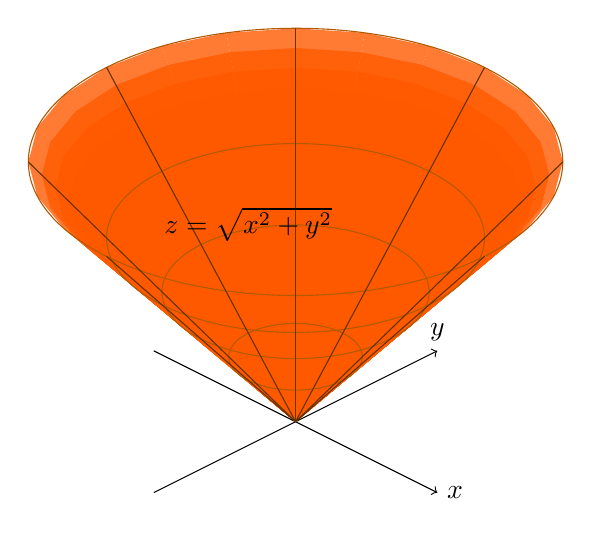
\begin{tikzpicture}[x={(0.8cm,-0.4cm)}, y={(0.8cm,0.4cm)}, z={(0cm,1.1cm)}, scale=1.5]
    % Draw axes
    \draw[->] (-1.5,0,0) -- (1.5,0,0) node[right] {$x$};
    \draw[->] (0,-1.5,0) -- (0,1.5,0) node[above] {$y$};
    \draw[->] (0,0,0) -- (0,0,2.5) node[above] {$z$};
    
    % Draw solid cone
    \foreach \z in {0.1,0.2,...,2} {
        \pgfmathsetmacro{\radius}{\z}
        \foreach \theta in {0,15,...,345} {
            \pgfmathsetmacro{\thetanext}{\theta+15}
            \pgfmathsetmacro{\xa}{\radius*cos(\theta)}
            \pgfmathsetmacro{\ya}{\radius*sin(\theta)}
            \pgfmathsetmacro{\xb}{\radius*cos(\thetanext)}
            \pgfmathsetmacro{\yb}{\radius*sin(\thetanext)}
            \fill[orange!70!red, opacity=0.8] (0,0,0) -- (\xa,\ya,\z) -- (\xb,\yb,\z) -- cycle;
        }
    }
    
    % Draw boundary circles
    \foreach \z in {0.5,1,1.414,2} {
        \draw[orange!70!black, thin, domain=0:360, samples=60, smooth, variable=\t] 
            plot ({\z*cos(\t)}, {\z*sin(\t)}, {\z});
    }
    
    % Draw generating lines
    \foreach \theta in {0,45,...,315} {
        \draw[orange!40!black, thin] (0,0,0) -- ({2*cos(\theta)}, {2*sin(\theta)}, 2);
    }
    
    % Label
    \node at (0, -0.5, 1.7) {$z=\sqrt{x^2+y^2}$};
\end{tikzpicture}
\end{center}

\textbf{The Sphere:} $x^2 + y^2 + z^2 = 4$ (radius 2, centered at origin)

\begin{center}
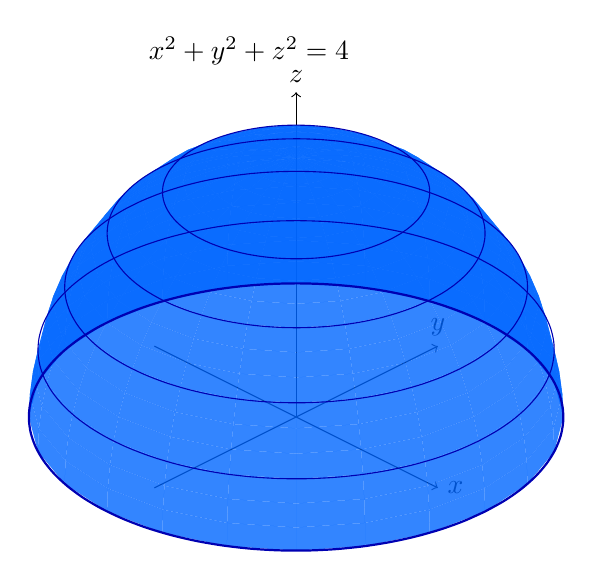
\begin{tikzpicture}[x={(0.8cm,-0.4cm)}, y={(0.8cm,0.4cm)}, z={(0cm,1.1cm)}, scale=1.5]
    % Draw axes
    \draw[->] (-1.5,0,0) -- (1.5,0,0) node[right] {$x$};
    \draw[->] (0,-1.5,0) -- (0,1.5,0) node[above] {$y$};
    \draw[->] (0,0,0) -- (0,0,2.5) node[above] {$z$};
    
    % Draw solid upper hemisphere
    \foreach \phi in {0,5,...,85} {
        \pgfmathsetmacro{\phinext}{\phi+5}
        \pgfmathsetmacro{\ra}{2*sin(\phi)}
        \pgfmathsetmacro{\za}{2*cos(\phi)}
        \pgfmathsetmacro{\rb}{2*sin(\phinext)}
        \pgfmathsetmacro{\zb}{2*cos(\phinext)}
        \foreach \theta in {0,15,...,345} {
            \pgfmathsetmacro{\thetanext}{\theta+15}
            \pgfmathsetmacro{\xa}{\ra*cos(\theta)}
            \pgfmathsetmacro{\ya}{\ra*sin(\theta)}
            \pgfmathsetmacro{\xb}{\rb*cos(\theta)}
            \pgfmathsetmacro{\yb}{\rb*sin(\theta)}
            \pgfmathsetmacro{\xc}{\rb*cos(\thetanext)}
            \pgfmathsetmacro{\yc}{\rb*sin(\thetanext)}
            \pgfmathsetmacro{\xd}{\ra*cos(\thetanext)}
            \pgfmathsetmacro{\yd}{\ra*sin(\thetanext)}
            \fill[blue!60!cyan, opacity=0.8] (\xa,\ya,\za) -- (\xb,\yb,\zb) -- (\xc,\yc,\zb) -- (\xd,\yd,\za) -- cycle;
        }
    }
    
    % Draw latitude circles
    \foreach \phi in {30,45,60,75} {
        \pgfmathsetmacro{\r}{2*sin(\phi)}
        \pgfmathsetmacro{\z}{2*cos(\phi)}
        \draw[blue!70!black, thin, domain=0:360, samples=60, smooth, variable=\t] 
            plot ({\r*cos(\t)}, {\r*sin(\t)}, {\z});
    }
    
    % Draw equator
    \draw[blue!70!black, thick, domain=0:360, samples=60, smooth, variable=\t] 
        plot ({2*cos(\t)}, {2*sin(\t)}, 0);
    
    % Label
    \node at (0, -0.5, 3) {$x^2+y^2+z^2=4$};
\end{tikzpicture}
\end{center}

\textbf{The Intersection Region:} Between cone (below) and sphere (above)

\begin{center}
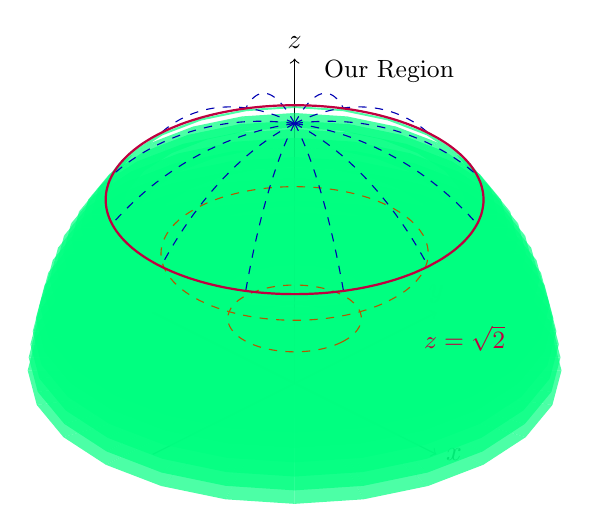
\begin{tikzpicture}[x={(0.8cm,-0.4cm)}, y={(0.8cm,0.4cm)}, z={(0cm,1.1cm)}, scale=1.5]
    % Draw axes
    \draw[->] (-1.5,0,0) -- (1.5,0,0) node[right] {$x$};
    \draw[->] (0,-1.5,0) -- (0,1.5,0) node[above] {$y$};
    \draw[->] (0,0,0) -- (0,0,2.5) node[above] {$z$};
    
    % Fill the solid region between cone and sphere
    % For z from 0 to sqrt(2), radius is z (cone constraint)
    \foreach \z in {0.1,0.2,...,1.414} {
        \pgfmathsetmacro{\radius}{\z}
        \foreach \theta in {0,15,...,345} {
            \pgfmathsetmacro{\thetanext}{\theta+15}
            \pgfmathsetmacro{\xa}{\radius*cos(\theta)}
            \pgfmathsetmacro{\ya}{\radius*sin(\theta)}
            \pgfmathsetmacro{\xb}{\radius*cos(\thetanext)}
            \pgfmathsetmacro{\yb}{\radius*sin(\thetanext)}
            \pgfmathsetmacro{\rsphere}{sqrt(4-\z*\z)}
            \pgfmathsetmacro{\xc}{\rsphere*cos(\theta)}
            \pgfmathsetmacro{\yc}{\rsphere*sin(\theta)}
            \pgfmathsetmacro{\xd}{\rsphere*cos(\thetanext)}
            \pgfmathsetmacro{\yd}{\rsphere*sin(\thetanext)}
            % Fill the annular region at height z
            \fill[green!50!cyan, opacity=0.7] (\xa,\ya,\z) -- (\xb,\yb,\z) -- (\xd,\yd,\z) -- (\xc,\yc,\z) -- cycle;
        }
    }
    
    % Draw cone surface (transparent)
    \foreach \z in {0.5,1,1.414} {
        \draw[orange!70!black, dashed, thin, domain=0:360, samples=60, smooth, variable=\t] 
            plot ({\z*cos(\t)}, {\z*sin(\t)}, {\z});
    }
    
    % Draw sphere surface (transparent)
    \foreach \theta in {0,30,...,330} {
        \draw[blue!70!black, dashed, thin, domain=0:1.414, samples=30, smooth, variable=\r] 
            plot ({\r*cos(\theta)}, {\r*sin(\theta)}, {sqrt(4-\r*\r)});
    }
    
    % Draw intersection circle at z = sqrt(2)
    \pgfmathsetmacro{\zint}{1.414}
    \pgfmathsetmacro{\rint}{1.414}
    \draw[thick, purple, domain=0:360, samples=60, smooth, variable=\t] 
        plot ({\rint*cos(\t)}, {\rint*sin(\t)}, {\zint});
    
    % Label
    \node at (.5, 0.5, 2.4) {\small Our Region};
    \node[purple] at (1.8, 0, 1) {\small $z=\sqrt{2}$};
\end{tikzpicture}
\end{center}

\textbf{Step 1: Understanding the Cartesian Challenge}

The cone and sphere intersect where $z = \sqrt{x^2+y^2}$ and $x^2+y^2+z^2=4$.

Substituting: $x^2+y^2+(\sqrt{x^2+y^2})^2 = 4$, so $2(x^2+y^2) = 4$, giving $x^2+y^2 = \answer{2}$.

At the intersection: $z = \sqrt{2}$ and the circle has radius $\sqrt{2}$.

\textbf{In Cartesian coordinates with order $dz\,dy\,dx$:}

For fixed $(x,y)$ with $x^2+y^2 \leq 2$:
$$\sqrt{x^2+y^2} \leq z \leq \sqrt{4-x^2-y^2}$$

For fixed $x$: $-\sqrt{2-x^2} \leq y \leq \sqrt{2-x^2}$

Overall: $-\sqrt{2} \leq x \leq \sqrt{2}$

$$M = \int_{-\sqrt{2}}^{\sqrt{2}} \int_{-\sqrt{2-x^2}}^{\sqrt{2-x^2}} \int_{\sqrt{x^2+y^2}}^{\sqrt{4-x^2-y^2}} z\,dz\,dy\,dx$$

This is quite messy! Square roots everywhere, and the bounds depend on each other in complicated ways.

\textbf{Step 2: Recognizing the Pattern}

What features suggest a better coordinate system?
\begin{selectAll}
    \choice[correct]{The sphere equation is $x^2 + y^2 + z^2 = 4$ (radial from origin)}
    \choice[correct]{The cone equation involves $\sqrt{x^2 + y^2}$ (cylindrical symmetry)}
    \choice[correct]{Both surfaces are centered at the origin}
    \choice{The region is rectangular}
\end{selectAll}

For a sphere centered at the origin, which coordinate system is best?
\begin{multipleChoice}
    \choice{Cartesian}
    \choice{Cylindrical}
    \choice[correct]{Spherical}
\end{multipleChoice}

\textbf{Step 3: The Spherical Coordinate Transformation}

Spherical coordinates $(\rho, \phi, \theta)$ relate to Cartesian via:
\begin{align*}
x &= \rho\sin\phi\cos\theta\\
y &= \rho\sin\phi\sin\theta\\
z &= \rho\cos\phi
\end{align*}

where:
\begin{itemize}
    \item $\rho \geq 0$ is the distance from the origin
    \item $0 \leq \phi \leq \pi$ is the angle down from the positive $z$-axis
    \item $0 \leq \theta < 2\pi$ is the azimuthal angle (same as cylindrical)
\end{itemize}

Key relation: $x^2 + y^2 + z^2 = \answer{\rho^2}$

The volume element transforms: $dV = \answer{\rho^2 \sin\phi}\,d\rho\,d\phi\,d\theta$

\textbf{Step 4: Transform the Surfaces}

\textbf{The sphere:} $x^2 + y^2 + z^2 = 4$ becomes $\rho^2 = 4$, so $\rho = \answer{2}$

This is beautiful! A constant bound.

\textbf{The cone:} $z = \sqrt{x^2 + y^2}$

Using $z = \rho\cos\phi$ and $\sqrt{x^2+y^2} = \rho\sin\phi$:
$$\rho\cos\phi = \rho\sin\phi$$

Dividing by $\rho$: $\cos\phi = \sin\phi$, so $\tan\phi = 1$, giving $\phi = \answer{\pi/4}$

The cone is a constant angle! The region is between the cone ($\phi = \pi/4$) and the north pole ($\phi = 0$).

So: $0 \leq \phi \leq \answer{\pi/4}$

\textbf{Step 5: Transform the Density}

The density was $\rho(x,y,z) = z$

In spherical coordinates: $z = \rho\cos\phi$

So the density becomes: $\rho(\rho,\phi,\theta) = \answer{\rho\cos\phi}$

(Note: We're using $\rho$ for both the density function and the spherical coordinate. Context makes it clear!)

\textbf{Step 6: Set Up the Integral in Spherical Coordinates}

The bounds are:
\begin{itemize}
    \item $0 \leq \rho \leq 2$ (from origin to sphere)
    \item $0 \leq \phi \leq \pi/4$ (from $z$-axis to cone)
    \item $0 \leq \theta \leq 2\pi$ (full rotation)
\end{itemize}

$$M = \int_{\answer{0}}^{\answer{2\pi}} \int_{\answer{0}}^{\answer{\pi/4}} \int_{\answer{0}}^{\answer{2}} (\rho\cos\phi) \cdot \rho^2\sin\phi\,d\rho\,d\phi\,d\theta$$

Simplifying: 
$$M = \int_0^{2\pi} \int_0^{\pi/4} \int_0^2 \rho^3\cos\phi\sin\phi\,d\rho\,d\phi\,d\theta$$

\textbf{Step 7: Evaluate the Integral}

The variables separate! Let's do each integral:

\textbf{Inner integral ($\rho$):}
$$\int_0^2 \rho^3\,d\rho = \left[\frac{\rho^4}{4}\right]_0^2 = \frac{16}{4} = \answer{4}$$

\textbf{Middle integral ($\phi$):}
$$\int_0^{\pi/4} \cos\phi\sin\phi\,d\phi = \int_0^{\pi/4} \frac{1}{2}\sin(2\phi)\,d\phi$$
$$= \frac{1}{2}\left[-\frac{1}{2}\cos(2\phi)\right]_0^{\pi/4} = -\frac{1}{4}[\cos(\pi/2) - \cos(0)]$$
$$= -\frac{1}{4}[0 - 1] = \answer{1/4}$$

\textbf{Outer integral ($\theta$):}
$$\int_0^{2\pi} d\theta = \answer{2\pi}$$

\textbf{Final answer:}
$$M = 4 \cdot \frac{1}{4} \cdot 2\pi = \answer{2\pi}$$

\begin{feedback}
Compare the two approaches! In Cartesian coordinates, we had:
\begin{itemize}
    \item Square root bounds: $-\sqrt{2-x^2} \leq y \leq \sqrt{2-x^2}$
    \item Nested dependence of bounds
    \item Complex expressions like $\sqrt{4-x^2-y^2}$
\end{itemize}

In spherical coordinates, we had:
\begin{itemize}
    \item Constant bounds: $0 \leq \rho \leq 2$, $0 \leq \phi \leq \pi/4$, $0 \leq \theta \leq 2\pi$
    \item Separable integral
    \item The sphere became $\rho = 2$ (one equation!)
    \item The cone became $\phi = \pi/4$ (one equation!)
\end{itemize}

This is the power of choosing the right coordinate system! The geometry of the problem guides us to the natural coordinates.
\end{feedback}
\end{problem}


\section*{Choosing the Right Coordinate System}

\begin{problem}
Match each region type with the best coordinate system:

For a cylinder aligned with the $z$-axis:
\begin{multipleChoice}
    \choice{Rectangular}
    \choice[correct]{Cylindrical}
    \choice{Spherical}
\end{multipleChoice}

For a sphere centered at the origin:
\begin{multipleChoice}
    \choice{Rectangular}
    \choice{Cylindrical}
    \choice[correct]{Spherical}
\end{multipleChoice}

For a rectangular box:
\begin{multipleChoice}
    \choice[correct]{Rectangular}
    \choice{Cylindrical}
    \choice{Spherical}
\end{multipleChoice}

For a cone:
\begin{multipleChoice}
    \choice{Rectangular}
    \choice{Cylindrical}
    \choice[correct]{Either cylindrical or spherical work well}
\end{multipleChoice}

\begin{feedback}
Choose coordinates that match your region's symmetry! This makes bounds simpler and integrals easier to evaluate.
\end{feedback}
\end{problem}


\end{document}
